%%%%%%%%%%%%%%%%%%%%%%%%%%%%%%%%%%%%%%%%%%%%%%%%%%%%%%%%%%%%%%%%%%%%%%%%

%%% LaTeX Template for AAMAS-2026 (based on sample-sigconf.tex)
%%% Prepared by the AAMAS-2026 Publication Chairs based on the version from AAMAS-2025. 

%%%%%%%%%%%%%%%%%%%%%%%%%%%%%%%%%%%%%%%%%%%%%%%%%%%%%%%%%%%%%%%%%%%%%%%%

%%% Start your document with the \documentclass command.


%%% == IMPORTANT ==
%%% Use the first variant below for the final paper (including author information).
%%% Use the second variant below to anonymize your submission (no author information shown).
%%% For further information on anonymity and double-blind reviewing, 
%%% please consult the call for paper information
%%% https://cyprusconferences.org/aamas2026/submission-instructions/

%%%% For anonymized submission, use this
\documentclass[sigconf,anonymous]{aamas} 

%%%% For camera-ready, use this
%\documentclass[sigconf]{aamas} 


%%% Load required packages here (note that many are included already).

\usepackage{balance} % for balancing columns on the final page
\usepackage{amsmath}
\usepackage{amsthm}
\usepackage{algorithm}
\usepackage{algpseudocode}
\algnewcommand{\LComment}[1]{\Statex \(\triangleright\)\ #1} % unnumbered full-line comment
\newtheorem{remark}{Remark}
\newcommand{\br}{br}
\newcommand{\argmax}{argmax}
\newcommand{\reg}{reg}
\newcommand{\cbr}{CBR}
%%%%%%%%%%%%%%%%%%%%%%%%%%%%%%%%%%%%%%%%%%%%%%%%%%%%%%%%%%%%%%%%%%%%%%%%

%%% AAMAS-2026 copyright block (do not change!)

\setcopyright{ifaamas}
\acmConference[AAMAS '26]{Proc.\@ of the 25th International Conference
on Autonomous Agents and Multiagent Systems (AAMAS 2026)}{May 25 -- 29, 2026}
{Paphos, Cyprus}{C.~Amato, L.~Dennis, V.~Mascardi, J.~Thangarajah (eds.)}
\copyrightyear{2026}
\acmYear{2026}
\acmDOI{}
\acmPrice{}
\acmISBN{}


%%%%%%%%%%%%%%%%%%%%%%%%%%%%%%%%%%%%%%%%%%%%%%%%%%%%%%%%%%%%%%%%%%%%%%%%

%%% == IMPORTANT ==
%%% Use this command to specify your submission number.
%%% In anonymous mode, it will be printed on the first page.

\acmSubmissionID{<<submission id>>}

%%% Use this command to specify the title of your paper.

\title[Counterfactual Credit Assignment in Empirical Metagame Analysis]{Counterfactual Credit Assignment in Empirical Metagame Analysis}

%%% Provide names, affiliations, and email addresses for all authors.

\author{Arthur Pendragon}
\affiliation{
\institution{Camelot Castle}
\city{Camelot}
\country{United Kingdom}}
\email{king.arthur@camelot.uk}

\author{Nimue}
\affiliation{
\institution{The Lady's Lake}
\city{Avalon}
\country{United Kingdom}}
\email{lady.of.the.lake@avalon.uk}

%%% Use this environment to specify a short abstract for your paper.

\begin{abstract}
This document outlines the formatting instructions for submissions to
AAMAS-2026. You can use its source file as a template when writing 
your own paper. It is based on the file `\texttt{sample-sigconf.tex}'
distributed with the ACM article template for \LaTeX\@.
\end{abstract}

%%% Use this command to specify a few keywords describing your work.
%%% Keywords should be separated by commas.

\keywords{general evaluation, multitask evaluation, empirical game-theoretic analysis}

%%%%%%%%%%%%%%%%%%%%%%%%%%%%%%%%%%%%%%%%%%%%%%%%%%%%%%%%%%%%%%%%%%%%%%%%

%%% Include any author-defined commands here.
     
\newcommand{\BibTeX}{\rm B\kern-.05em{\sc i\kern-.025em b}\kern-.08em\TeX}

%%%%%%%%%%%%%%%%%%%%%%%%%%%%%%%%%%%%%%%%%%%%%%%%%%%%%%%%%%%%%%%%%%%%%%%%

\begin{document}

%%% The following commands remove the headers in your paper. For final 
%%% papers, these will be inserted during the pagination process.

\pagestyle{fancy}
\fancyhead{}

%%% The next command prints the information defined in the preamble.

\maketitle 

%%%%%%%%%%%%%%%%%%%%%%%%%%%%%%%%%%%%%%%%%%%%%%%%%%%%%%%%%%%%%%%%%%%%%%%%

\section{Introduction}
Artificial intelligence is becoming part of the fabric of society, with autonomous agents increasingly acting on our behalf in markets, negotiations, and online platforms. These settings are rarely purely cooperative or purely competitive; they are \emph{mixed-motive}, combining shared and conflicting interests, so that elements of cooperation and competition appear together almost everywhere agents interact. As capable agents are deployed into them, what matters is not only how well an agent performs on its own, but how it shapes the social character of the outcomes it takes part in---whether its presence makes collective outcomes more cooperative and higher in welfare, or less. Measuring these cooperative and social-welfare properties of an agent in general mixed-motive settings is a challenge that has drawn sustained attention.

\begin{figure*}[t]
\centering
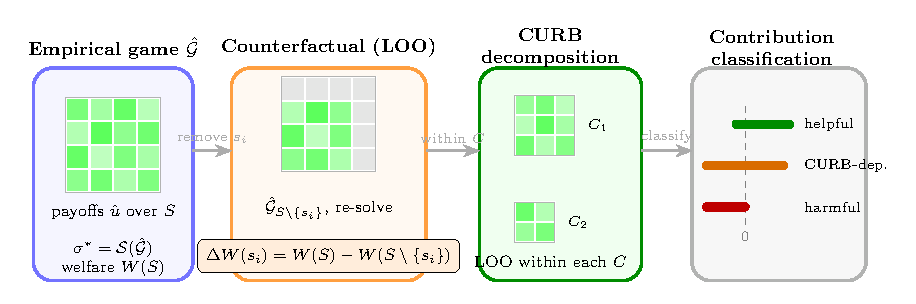
\includegraphics[width=\textwidth]{framework_figure.pdf}
\caption{\textbf{Counterfactual meta-game analysis.} From an empirical game $\hat{\mathcal{G}}$ over a strategy set $S$ (left), we measure each strategy's counterfactual contribution to the equilibrium outcome by leave-one-out: removing the strategy, re-solving, and comparing the resulting social metric (centre-left). Repeating this \emph{within} the game's CURB sets---minimal strategy subsets closed under best responses, which chart its equilibrium landscape (centre-right)---gives each strategy an interval of effects across strategic contexts, classifying it as robustly welfare-improving, robustly welfare-reducing, or context-dependent (right).}
\label{fig:framework}
\end{figure*}

This challenge sits at the heart of the cooperative-AI agenda. \citet{dafoe2021cooperative} argue that learning to find common ground is a defining problem for AI, and \citet{Du2023ARO} survey the mechanisms by which cooperation is promoted or undermined across multi-agent learning. A recurring lesson is that individual capability and collective outcome can come apart: \citet{conitzer2023foundations} show that agents which are individually well aligned with a social objective can nonetheless steer a system toward worse equilibria than would arise without them. Cooperativeness, then, is a property of how agents jointly shape one another's incentives, not a quantity any single agent carries on its own---and so it must be measured in strategic context.

Empirical game-theoretic analysis (EGTA) \citep{wellman2025empirical} supplies exactly this context. Its meta-game form \citep{Li2024AME, smithline2025measuring} treats each agent as a strategy in an empirical game estimated from cross-play and solves for a Nash equilibrium, which serves as a prediction of how the strategies would be played against one another in practice. Metagame analysis then evaluates each agent relative to that equilibrium, scoring its performance and its social metrics---welfare, fairness, cooperation. The equilibrium is, in effect, the reference against which agents are judged, and that reference has social qualities of its own: it is more or less cooperative, more or less efficient. Standard analysis treats this reference as fixed, even though the strategy set that induces it is somewhat ad hoc---whatever agents researchers happened to assemble---and an empirical game typically admits several equilibria. This invites a counterfactual question about the reference itself.

We extend empirical meta-game analysis along this counterfactual axis (Figure~\ref{fig:framework}). Rather than only scoring each strategy against a fixed equilibrium, we ask what each strategy \emph{contributes} to the equilibrium outcome of the full game---how the equilibrium, and the cooperation, welfare, and fairness realized at it, would change were the strategy not available---and read that contribution as the social character the strategy brings to the system. Because an empirical game can admit many equilibria, we further decompose it into its CURB sets \citep{Basu1991StrategySC}: minimal strategy subsets closed under best responses, which chart the equilibrium landscape of the game (every equilibrium lies inside one) and expose structural facts about it, letting us measure each strategy's contribution within strategically coherent contexts rather than under a single equilibrium selection. This reframes evaluation from ``how does a strategy perform at equilibrium?'' to:

\textbf{RQ.} \textit{What is each strategy's contribution to the cooperation and welfare realized at the empirical-game equilibrium?}

\begin{itemize}
\item \textbf{Counterfactual meta-game analysis.} We extend empirical meta-game evaluation by varying the strategy set rather than treating it as fixed, measuring each strategy's counterfactual contribution to equilibrium social metrics as strategies are added or removed. This shifts the unit of evaluation from a strategy's performance at a fixed equilibrium to its effect on the equilibrium outcome---a property of the game structure, not of the strategy in isolation.                                                                                      
\item \textbf{CURB-conditional robustness.} Because an empirical game admits many equilibria, we make the counterfactual robust to equilibrium selection by computing it within CURB sets \citep{Basu1991StrategySC}---strategically self-reinforcing subsets that are epistemically stable under mutual belief in rationality \citep{asheim2016epistemically}---and classify each strategy as robustly welfare-improving, robustly welfare-reducing, or context-dependent.

\item \textbf{Multi-domain evaluation.} We apply the framework to multi-agent bargaining with RL and LLM strategies \citep{smithline2025measuring} and to the iterated Prisoner's Dilemma using Axelrod-library strategies, showing it generalizes across domains with different strategic structure.                                
\end{itemize}

\section{Background}

\subsection{Related Work}

\paragraph{Individual and pairwise evaluation.} The dominant evaluation paradigm scores agents in isolation: single-agent benchmarks measure task performance with no strategic context, while rating systems such as Elo and its successors score agents by pairwise outcomes. \citet{Balduzzi2018ReevaluatingE} decompose payoff matrices into transitive and cyclic components, \citet{bertrand2023limitations} show that Elo fails on intransitive games and propose a decomposition of $\mathrm{logit}(P)$ that recovers the transitive backbone, and \citet{marris2025deviation} give a clone-invariant rating under correlated equilibria. These methods answer \emph{how strong} an agent is relative to others; they do not ask what an agent's presence does to the system.

\paragraph{Cooperation and welfare in multi-agent systems.} A second line studies cooperation directly. Sequential social dilemmas \citep{leibo2017multiagent} and the surrounding literature \citep{Du2023ARO} design environments in which cooperative behavior can emerge, and cooperation has been called a central challenge for AI \citep{dafoe2021cooperative, Dafoe2020OpenPI}. \citet{conitzer2023foundations} expose the core difficulty for evaluation: individually well-aligned agents can still produce poor equilibria, so the cooperativeness of an outcome is not reducible to individual agent quality. Yet most multi-agent benchmarks still score agents by their individual outcomes (welfare achieved, cooperation rate), evaluating each agent \emph{within} a fixed environment rather than asking how it shapes that environment.

\paragraph{Counterfactual measures.} Closest to our perspective are counterfactual measures of agent behavior. \citet{barnett2025measuring} measure the cooperativeness of an agent in a stochastic game counterfactually---contrasting realized group utility with what a purely self-interested agent would have attained---and \citet{foerster2018counterfactual} use a counterfactual baseline to assign credit among cooperating policies. Both apply the counterfactual at the level of an agent's \emph{actions} within a fixed game. We lift the counterfactual to the level of the \emph{strategy set}: rather than asking how an agent would have acted differently, we ask how the equilibrium would differ were the agent not available at all, re-solving the metagame in each case.

\paragraph{Empirical game-theoretic evaluation.} EGTA \citep{wellman2025empirical} evaluates agents at the equilibrium of an empirical game and has recently been adapted into a meta-game framework for evaluating capable AI \citep{Li2024AME, smithline2025measuring, Luo2026}; \citet{liu2025reevaluating} attribute within-equilibrium contributions to co-players at a fixed equilibrium. These approaches are strategically grounded but still ask ``how does each agent perform at equilibrium?'', treating the strategy set---and hence the equilibrium---as given. In practice, agent populations are not static: new models are continually added to leaderboards and evaluations, and adding an agent changes the game for every other agent in the pool. We therefore vary the strategy set and re-equilibrate, shifting the question from an agent's performance \emph{within} an equilibrium to its effect \emph{on} the equilibrium, and surfacing structural roles---substitutable, destabilizing, or reshaping the equilibrium from outside its support---that fixed-context evaluation cannot.

\paragraph{Closure-based solution concepts.} CURB sets \citep{Basu1991StrategySC} formalize strategy subsets closed under best responses; their minimal variants always exist, are computable in polynomial time for two-player games \citep{Benisch2010AlgorithmsFC, Klimm2009FindingAM}, admit an axiomatic characterization \citep{voorneveld2005axiomatization}, and are epistemically stable under mutual belief in rationality \citep{asheim2016epistemically}. Related closure and preparation (``prep'') concepts arise as the rest points of natural learning dynamics \citep{Hurkens1995LearningBF}. We use CURB sets not as a solution concept to be played, but as a decomposition of the empirical game that charts its equilibrium landscape and grounds the counterfactual analysis.



\subsection{Normal-Form Games}

A normal-form game $\mathcal{G} = (N, (S_i)_{i \in N}, (u_i)_{i \in N})$ comprises a finite set of players $N$, a non-empty set of strategies $S_i$
for each player $i \in N$, and a utility function $u_i : \prod_{j \in N} S_j \rightarrow \mathbb{R}$. A mixed strategy $\sigma_i \in \Delta(S_i)$ is
a probability distribution over $S_i$, where $\Delta(\cdot)$ denotes the simplex over a set. We denote the strategy profile of all players other than $i$ by $\sigma_{-i} = (\sigma_j)_{j \neq i}$. The joint mixed-strategy space is $\Delta(S) = \prod_{i \in N} \Delta(S_i)$.

We define the best-response correspondence for player $i$ as $\text{BR}_i(\sigma_{-i}) \equiv \arg\max_{\sigma_i' \in \Delta(S_i)} u_i(\sigma_i', \sigma_{-i})$, and the joint best-response correspondence as $\text{BR}(\sigma) \equiv \prod_{i \in N} \text{BR}_i(\sigma_{-i})$. A Nash equilibrium (NE) is a profile $\sigma^*$ such that $\sigma^* \in \text{BR}(\sigma^*)$. The regret of player $i$ at profile $\sigma$ in game $\mathcal{G}$ is defined as $\text{Reg}_i^{\mathcal{G}}(\sigma) \equiv \max_{s_i' \in S_i} u_i(s_i', \sigma_{-i}) - u_i(\sigma_i, \sigma_{-i})$, capturing the maximum improvement player $i$ can obtain by unilaterally deviating from $\sigma_i$. By definition, every player has zero regret at a Nash equilibrium. An $\epsilon$-NE is a profile where no player can improve by more than $\epsilon$. The total regret of a profile is $\text{Reg}^{\mathcal{G}}(\sigma) \equiv \sum_{i \in N} \text{Reg}_i^{\mathcal{G}}(\sigma)$.

\subsection{Empirical Games and Restricted Games}
A restricted game $\hat{\mathcal{G}}_{S \downarrow X}$ is a projection of the full game $\mathcal{G}$ in which players are constrained to strategy
subsets $X_i \subseteq S_i$. An empirical game $\hat{\mathcal{G}}$ is an estimate of $\mathcal{G}$ where payoffs $\hat{u}_i$ are estimated through
simulation. The restricted empirical game is denoted $\hat{\mathcal{G}}_{S \downarrow X} = (N, (X_i), (\hat{u}_i))$.

We denote the equilibrium solver (meta-strategy solver) by $\mathcal{S}$, which maps a game to an equilibrium mixture: $\sigma^*_X = \mathcal{S}(\hat{\mathcal{G}}_{S \downarrow X})$. A metric functional $\Phi$ evaluates a property of interest (welfare, fairness, cooperation) at an
equilibrium: $\Phi(\hat{\mathcal{G}}_{S \downarrow X}, \sigma^*_X)$. The restricted game value functional, making solver dependence explicit, is:
\begin{equation}
  W_{\mathcal{S}}(X) := \Phi(\hat{\mathcal{G}}_{S \downarrow X}, \mathcal{S}(\hat{\mathcal{G}}_{S \downarrow X}))
\end{equation}

\subsection{CURB Sets}

The conditional best response of a set $X \subseteq S$ is:
\begin{equation}
  \text{CBR}(X) = \{s_i \in S_i : \exists \sigma \in \Delta(X) \text{ s.t. } s_i \in \arg\max_{s_i' \in S_i} u_i(s_i', \sigma_{-i})\}
\end{equation}
the set of pure strategies that are best responses to some mixture over $X$. A set $X$ is \textit{Closed Under Rational Behavior} (CURB)
\citep{Basu1991StrategySC} if $\text{CBR}(X) \subseteq X$: every best response to any mixture over $X$ is already contained in $X$.  Minimal CURB (min-CURB) are CURB sets that do not contain any other CURB set within them, further these sets are disjoint, always exist in finite games, and can be computed in polynomial time for two-player normal-form games \citep{Benisch2010AlgorithmsFC, Klimm2009FindingAM}.  Its noted in \citep{Basu1991StrategySC} every Nash equilibrium of the game lives inside some curbset, but not every Nash equilibrium lives inside a minimal curb set. Further min-CURB sets are fixed under rational behavior (FURB) by definition.

\subsection{Strategy Removal and Equilibrium Stability}

The set of Nash equilibria satisfies contraction consistency
but not expansion consistency with respect to strategy removal.
If $\sigma^*$ is a NE of $\mathcal{G}$ with
$\text{supp}(\sigma^*) \subseteq X$, then $\sigma^*$ remains
a NE of the restricted game $\mathcal{G}_{S \downarrow X}$:
removing strategies outside the equilibrium support cannot
destabilize existing equilibria, as it only eliminates
potential deviations. However, the restricted game may admit
\textit{additional} equilibria not present in the full game,
because removing a strategy eliminates it as a profitable
deviation that was previously destabilizing other profiles.

This asymmetry has two consequences. First, the LOO effect
$\Delta W(s_i \mid X)$ captures both the solver selecting a
different persisting equilibrium (selection effect) and the
solver selecting a newly admissible equilibrium (expansion
effect). Second, point-valued equilibrium selection concepts
satisfying existence are provably inconsistent under game
transformations \citep{norde1996equilibrium}, meaning no
single-equilibrium selector provides stable counterfactual
comparisons. CURB sets avoid this problem as a set-valued
concept satisfying consistency
\citep{voorneveld2005axiomatization}.

\begin{lemma}[CURB stability under strategy removal]
Let $C$ be a CURB set of $\mathcal{G} = (N, (S_i), (u_i))$.
For any strategy $s_j \in S \setminus C$, $C$ remains a
CURB set of the restricted game
$\mathcal{G}_{S \downarrow S \setminus \{s_j\}}$.
\end{lemma}

\begin{proof}
Since $C$ is CURB in $\mathcal{G}$, we have
$\text{CBR}_{\mathcal{G}}(C) \subseteq C$. This means
no strategy outside $C$ is a best response to any
mixture over $C$; in particular, $s_j \notin C$ implies
$s_j \notin \text{CBR}_{\mathcal{G}}(C)$. Removing $s_j$ from the game does not alter the strategies in $C$ or the payoffs between them. In the restricted game $\mathcal{G}_{S \downarrow S \setminus \{s_j\}}$, the only change is that $s_j$ is no longer available as a potential deviation. For any $\sigma \in \Delta(C)$, the set of best
responses to $\sigma$ in the restricted game is $\text{BR}_{\mathcal{G}}(\sigma) \setminus \{s_j\}$: the same best responses as in the full game, minus $s_j$ which is no longer available. Since $s_j$ was never a best response to any mixture over $C$ (as $s_j \notin \text{CBR}_{\mathcal{G}}(C)$), this removal has no effect: $\text{BR}_{\mathcal{G}}(\sigma) \setminus \{s_j\} = \text{BR}_{\mathcal{G}}(\sigma) \subseteq \text{CBR}_{\mathcal{G}}(C) \subseteq C$. Taking the union over all $\sigma \in \Delta(C)$, we obtain $\text{CBR}_{\mathcal{G}_{S \downarrow S \setminus \{s_j\}}}(C) \subseteq C$. 
\end{proof}

\begin{remark}
By Lemma 1, removing strategy $s_i$ from the full game preserves every CURB set that does not contain $s_i$, along with their internal equilibria. In the CURB-conditional analysis, where LOO is performed within each CURB set independently, agents outside a CURB set have exactly zero effect on that CURB set's welfare. This justifies restricting the CURB-conditional LOO computation to CURB sets containing $s_i$.
\end{remark}

\subsection{A Worked Example}

Following \citet{smithline2025measuring}, we take their bargaining empirical game and apply our leave-one-out (LOO) decomposition. The maximum-entropy Nash equilibrium (MENE) of the full game places roughly $80\%$ of its mass on PPO and $20\%$ on PSRO; every other strategy has zero support. A standard analysis would stop here, reporting that two reinforcement-learning (RL) agents account for the entire equilibrium. The counterfactual decomposition tells a different story.

Throughout, we describe each strategy by the change its presence makes to a social metric at the equilibrium: a strategy whose presence lowers a metric is one whose removal would raise it.

\paragraph{An off-equilibrium agent that suppresses welfare.} Consider OpenAI~5.2-low, which has zero equilibrium support yet the highest individual social metrics in the pool. Its presence nonetheless \emph{lowers} every social metric at the equilibrium---utilitarian welfare by $10.87$, Nash welfare by $7.60$, advantage-Nash welfare by $4.41$, and the EF1$^+$ fairness rate by $7.7$ percentage points. Removing it shifts the MENE to $68\%$ PPO, $30\%$ OpenAI~5.4-medium, and $2\%$ PSRO. The mechanism is structural: 5.2-low is never played, but it is the best response to 5.4-medium, and its mere availability deters 5.4-medium from entering the equilibrium. An agent that looks individually excellent is, in equilibrium, holding welfare down---and its counterfactual effect is larger in magnitude than that of PPO, the $80\%$-support agent.

\paragraph{A high-support agent that is substitutable.} PPO carries most of the equilibrium mass yet has a near-zero LOO effect. Removing it shifts the MENE to $80\%$ MAPPO, $20\%$ PSRO: MAPPO is a functional clone, so the dominant agent is almost perfectly substitutable. Its individual prominence overstates its structural importance.

\paragraph{A low-support agent that pins the regime.} PSRO has only $20\%$ support but the largest effect of any agent: its presence lowers utilitarian welfare by $39.08$. Removing it collapses the equilibrium from RL-dominated to LLM-dominated ($44\%$ 5.4-medium, $33\%$ 5.2-low, $16\%$ 5.2-medium, $7\%$ 5.2-none). PSRO's presence is what forces the more competitive, lower-welfare equilibrium; like 5.2-low, it holds the current regime in place.

A standard metagame analysis would describe 5.2-low as a socially beneficial agent---it scores best on every social metric. But if its presence forces a lower-welfare equilibrium, is it really the cooperative one? This is the gap we address: practitioners typically treat the strategic context as fixed and evaluate agents within it. We add a layer that treats the equilibrium as something the agents collectively produce, and asks what each agent's presence contributes to the equilibrium being what it is.

\section{Methodology}

\subsection{Equilibrium Analysis}

Standard metagame analysis solves for an equilibrium on the full game and evaluates each agent's performance at it:
\begin{align}
  \sigma^*_X &= \mathcal{S}(\hat{\mathcal{G}}_{S \downarrow X}) \\
  W(X) &= \sigma^{*\top}_X \, M \, \sigma^*_X
\end{align}
This answers ``how does each agent perform at equilibrium?'', but treats the equilibrium---and the strategy set that induces it---as fixed.

\subsection{Counterfactual Leave-One-Out Analysis}

The core counterfactual operation removes an agent $s_i$ from the strategy set, re-solves for equilibrium, and measures the resulting change in a social metric:
\begin{equation}
  \Delta W(s_i \mid X) := W_{\mathcal{S}}(X) - W_{\mathcal{S}}(X \setminus \{s_i\})
\end{equation}
where both equilibria are found by the same solver $\mathcal{S}$. A negative $\Delta W$ means the agent's presence lowers the metric at equilibrium---removing it yields a higher value---while a positive $\Delta W$ means its presence raises it. Because $\sigma^* = \mathcal{S}(\hat{\mathcal{G}})$ is a non-linear function of the strategy set, $\Delta W(s_i \mid X)$ captures an agent's effect \emph{through} the equilibrium, including the effect of agents that themselves carry no equilibrium weight.

\subsection{CURB-Conditional Analysis}
\label{sec:curb-conditional}

Full-game LOO effects depend on the solver's equilibrium selection, and as Section~\ref{sec:exp-bargaining} shows, different solvers can select very different equilibria. To make the counterfactual analysis robust to this choice, we perform LOO \emph{within each CURB set}---a strategically coherent restricted game in which every Nash equilibrium is contained.

For each CURB set $C$ (found via \citet{Klimm2009FindingAM}, with Monte-Carlo sampling for non-minimal sets), we solve for the within-set equilibrium $\sigma^*_C = \mathcal{S}(\hat{\mathcal{G}}_{S \downarrow C})$, evaluate its welfare $W(C) = \sigma_C^{*\top} M[C, C]\,\sigma^*_C$, and compute the within-set LOO effect for each $s_i \in C$:
\begin{equation}
  \Delta(s_i \mid C) = W(C) - W(C \setminus \{s_i\}).
\end{equation}
Collecting these over all CURB sets containing $s_i$ yields the interval
\begin{equation}
  \big[\underline{\Delta}(s_i),\, \overline{\Delta}(s_i)\big]
  = \Big[\min_{C \ni s_i,\, |C| \geq 2} \Delta(s_i \mid C),\ \max_{C \ni s_i,\, |C| \geq 2} \Delta(s_i \mid C)\Big].
\end{equation}
We report this interval both on the point-estimate empirical game (Table~\ref{tab:curb-bargaining}) and, to quantify sampling uncertainty, as the mean and $95\%$ CI of each bound across bootstrap resamples (Figures~\ref{fig:curb-mene}--\ref{fig:curb-cce}).

\textbf{Classification.} We classify each agent by where this interval sits:
\begin{itemize}
  \item \textbf{Robustly helpful}: $\underline{\Delta}(s_i) > 0$ --- improves welfare in every CURB set it belongs to.
  \item \textbf{Robustly harmful}: $\overline{\Delta}(s_i) \leq 0$ and $\underline{\Delta}(s_i) < 0$ --- never improves welfare, and strictly reduces it in some context.
  \item \textbf{CURB-dependent}: $\underline{\Delta}(s_i) < 0 < \overline{\Delta}(s_i)$ --- its sign depends on the strategic context.
\end{itemize}
Because the interval ranges over strategic contexts rather than a single solver's selection, it exposes structural roles---substitutable, destabilizing, or context-dependent---that fixed-equilibrium evaluation cannot.

\subsection{The Full Procedure}
\label{sec:algorithm}

Algorithm~\ref{alg:cmga} ties the pieces together into the procedure we run in the experiments. The two analyses---equilibrium analysis (Level 1) and CURB-conditional counterfactual analysis (Level 3)---are computed inside a common bootstrap loop, over a set of solvers and a set of social metrics, so that every reported quantity carries a sampling interval and all quantities are \emph{paired} within each resample. Level 1 records how each agent performs \emph{at} an equilibrium; Level 3 records each agent's contribution \emph{through} the equilibrium, as the range of its within-CURB leave-one-out effect. Because the levels share resamples, comparisons between them (and across solvers) are made on common draws. The aggregation step turns the per-sample bounds into the confidence intervals plotted in Figures~\ref{fig:curb-mene}--\ref{fig:curb-cce} and the robust role labels.

\begin{algorithm*}[t]
\caption{Counterfactual Meta-Game Analysis (bootstrap, multi-solver, multi-metric)}
\label{alg:cmga}
\begin{algorithmic}[1]
\Require raw cross-play data; bootstrap count $B$; solvers $\{\mathcal{S}_1,\mathcal{S}_2,\dots\}$ (e.g.\ MENE, maxent-CCE); metrics $\{k_1,k_2,\dots\}$ (e.g.\ UW, NW, cooperation, fairness)
\Ensure per-agent equilibrium statistics and CURB-conditional intervals $[\underline{\Delta}(s_i),\overline{\Delta}(s_i)]$ with $95\%$ CIs and robust role labels
\Statex
\For{$b = 1$ \textbf{to} $B$}
  \State resample raw data $\rightarrow$ empirical game $\hat{\mathcal{G}}^{(b)}$ and metric matrices $\{\hat{M}^{(b)}_k\}_k$
  \Statex
  \LComment{\textbf{Level 1 --- equilibrium analysis:} performance \emph{at} a fixed equilibrium}
  \ForAll{solvers $\mathcal{S}\in\{\mathcal{S}_1,\mathcal{S}_2,\dots\}$}
    \State $\sigma^{*} \gets \mathcal{S}(\hat{\mathcal{G}}^{(b)})$
    \State $\forall\,k,\,s_i:\ $ record payoff, regret, and the metric-$k$ value of $s_i$ at $\sigma^{*}$ on $\hat{M}^{(b)}_k$
  \EndFor
  \Statex
  \LComment{\textbf{Level 3 --- CURB-conditional counterfactual:} contribution \emph{through} the equilibrium}
  \State $\mathcal{C} \gets \textsc{CurbSets}(\hat{\mathcal{G}}^{(b)})$ \Comment{best-response closed; independent of the solver}
  \ForAll{solvers $\mathcal{S}$ and agents $s_i \in S$}
    \For{each $C \in \mathcal{C}$ with $s_i \in C$ and $|C|\geq 2$}
      \State $\sigma^{*}_C \gets \mathcal{S}(\hat{\mathcal{G}}^{(b)}_{S\downarrow C})$,\quad $\sigma^{*}_{C\setminus i} \gets \mathcal{S}(\hat{\mathcal{G}}^{(b)}_{S\downarrow C\setminus\{s_i\}})$
      \State $\forall\,k:\ \Delta_k(s_i\mid C,b) \gets \sigma_C^{*\top}\hat{M}^{(b)}_k[C,C]\,\sigma^{*}_C \;-\; \sigma_{C\setminus i}^{*\top}\hat{M}^{(b)}_k[C',C']\,\sigma^{*}_{C\setminus i}$ \Comment{$C'=C\setminus\{s_i\}$}
    \EndFor
    \State $\forall\,k:\ \underline{\Delta}^{(b)}_k(s_i) \gets \min_{C}\Delta_k(s_i\mid C,b)$,\quad $\overline{\Delta}^{(b)}_k(s_i) \gets \max_{C}\Delta_k(s_i\mid C,b)$
  \EndFor
\EndFor
\Statex
\LComment{\textbf{Aggregate across the $B$ paired resamples}}
\State compute $95\%$ CIs for all Level-1 and Level-3 quantities; record CURB-set survival frequency across $b$
\ForAll{agents $s_i \in S$ and metrics $k$}
  \If{$\mathrm{CI}_{\mathrm{lo}}\big[\underline{\Delta}_k(s_i)\big] > 0$} \State label $s_i$ \textbf{robustly helpful} for $k$
  \ElsIf{$\mathrm{CI}_{\mathrm{hi}}\big[\overline{\Delta}_k(s_i)\big] < 0$} \State label $s_i$ \textbf{robustly harmful} for $k$
  \Else{} \State label $s_i$ \textbf{CURB-dependent} for $k$
  \EndIf
\EndFor
\State \Return per-agent equilibrium statistics and intervals with CIs and labels \Comment{paired across $b$ $\Rightarrow$ direct comparisons valid}
\end{algorithmic}
\end{algorithm*}

\section{Experiments}
\label{sec:experiments}

We demonstrate counterfactual meta-game analysis on a bargaining empirical game over indivisible items \citep{smithline2025measuring}.
% PD (Axelrod) experiments to be added once the L1/L2/L3 pipeline is run on the
% 224-strategy tournament with the cooperation matrix as a second welfare metric.

\subsection{Bargaining}
\label{sec:exp-bargaining}

\paragraph{Setup.} The empirical game has 13 strategies spanning three families: reinforcement-learning agents (PPO, PSRO, MAPPO, NFSP), large language model (LLM) agents (the OpenAI 5.2 and 5.4 families at several decoding temperatures), and classical heuristics (walk-away, tough, soft, an EF1 bargainer, and an aspiration bargainer). Payoffs are estimated from the cross-play rollouts of \citet{smithline2025measuring}. We evaluate five social metrics at equilibrium: utilitarian welfare (UW), Nash welfare (NW), advantage-Nash welfare (NW$^+$), and two envy-freeness rates (EF1, EF1$^+$).

\paragraph{The equilibrium depends on the solver.} The maximum-entropy Nash equilibrium (MENE) of the full game places $80\%$ of its mass on PPO and $20\%$ on PSRO; every other strategy has zero support. The maximum-entropy coarse-correlated equilibrium (CCE) of the \emph{same} game is instead dominated by LLM strategies (OpenAI 5.4-medium $\approx 35\%$, 5.2-none $\approx 23\%$, 5.2-low $\approx 22\%$, with the remainder spread over other LLM variants). The choice of solution concept alone flips which family of agents appears to ``win'' the game. This fragility is precisely why we attribute outcomes through counterfactuals rather than through a single equilibrium, and why our CURB-conditional analysis ranges over strategically coherent subgames rather than committing to one solver's selection.

\paragraph{CURB-conditional classification.} Table~\ref{tab:curb-bargaining} reports, for each agent, the range of its leave-one-out welfare effect taken over the CURB sets that contain it (under MENE, on the average game, which has 23 CURB sets). Because the range is over strategic contexts rather than over bootstrap resamples, it is unaffected by the equilibrium-selection noise that makes single-solver leave-one-out estimates unstable.

\begin{table}[t]
\caption{CURB-conditional leave-one-out on the bargaining average game (MENE). Each cell is the range $[\min_C \Delta, \max_C \Delta]$ of an agent's LOO welfare effect over the CURB sets containing it (sign convention $\Delta W = W(X) - W(X\setminus\{s_i\})$). PPO improves welfare in every context; PSRO's sign depends on context; MAPPO and 5.2-low never improve welfare. Agents not shown have negligible effect across all CURB sets.}
\label{tab:curb-bargaining}
\small
\begin{tabular}{lccc l}
\hline
Agent & UW & NW$^+$ & EF1$^+$ & Class \\
\hline
PPO     & $[+6.3,\,+6.3]$ & $[+2.0,\,+2.0]$ & $[+.01,\,+.01]$ & helpful \\
PSRO    & $[-45.3,\,+6.7]$ & $[-14.0,\,+3.4]$ & $[-.28,\,+.01]$ & dependent \\
MAPPO   & $[-3.6,\,0]$ & $[-0.4,\,0]$ & $[-.02,\,0]$ & harmful \\
5.2-low & $[-46.9,\,0]$ & $[-4.4,\,0]$ & $[-.08,\,0]$ & harmful \\
\hline
\end{tabular}
\end{table}

Table~\ref{tab:curb-bargaining} resolves the puzzle of the worked example. PPO, the high-support agent, is \emph{robustly helpful}: its LOO effect is identically $+6.3$ UW across all sixteen CURB sets it belongs to, a stable, context-independent contribution. PSRO is the only \emph{CURB-dependent} agent: its UW effect ranges from $-45.3$ to $+6.7$, so whether its presence helps or harms welfare depends entirely on which strategically coherent subgame it is evaluated within---a structural role that fixed-equilibrium evaluation cannot expose. MAPPO and OpenAI 5.2-low never improve welfare in any CURB set; their effect is at most zero. In particular 5.2-low, which has the highest individual social metrics in the pool, is robustly welfare-\emph{reducing} once strategic context is taken into account: it is the cooperative-looking agent whose presence holds welfare down.

\paragraph{Robustness across resamples and solvers.} To check that this picture is neither an artifact of the point estimate nor of a particular solver, we recompute the CURB-conditional intervals across bootstrap resamples of the empirical game, under both MENE (Figure~\ref{fig:curb-mene}) and maximum-entropy CCE (Figure~\ref{fig:curb-cce}). For each agent and metric we plot the mean and $95\%$ CI of the per-sample lower bound $\underline{\Delta}$ (red) and upper bound $\overline{\Delta}$ (green). Two observations stand out. First, the qualitative role structure is stable: the LLM strategies (5.4-medium, 5.2-none, 5.2-low) carry positive upper bounds---they raise welfare in some strategically coherent contexts---while PSRO and MAPPO carry negative lower bounds, and the heuristics sit at zero. Second, and more telling, this structure is the \emph{same} under both solvers, even though MENE and CCE select very different point equilibria (RL-dominated versus LLM-dominated). The CURB-conditional analysis is thus robust to the equilibrium-selection choice that destabilizes single-equilibrium evaluation; the width of the confidence intervals reflects that sampling uncertainty, not a change in the qualitative attribution.

\begin{figure*}[t]
\centering
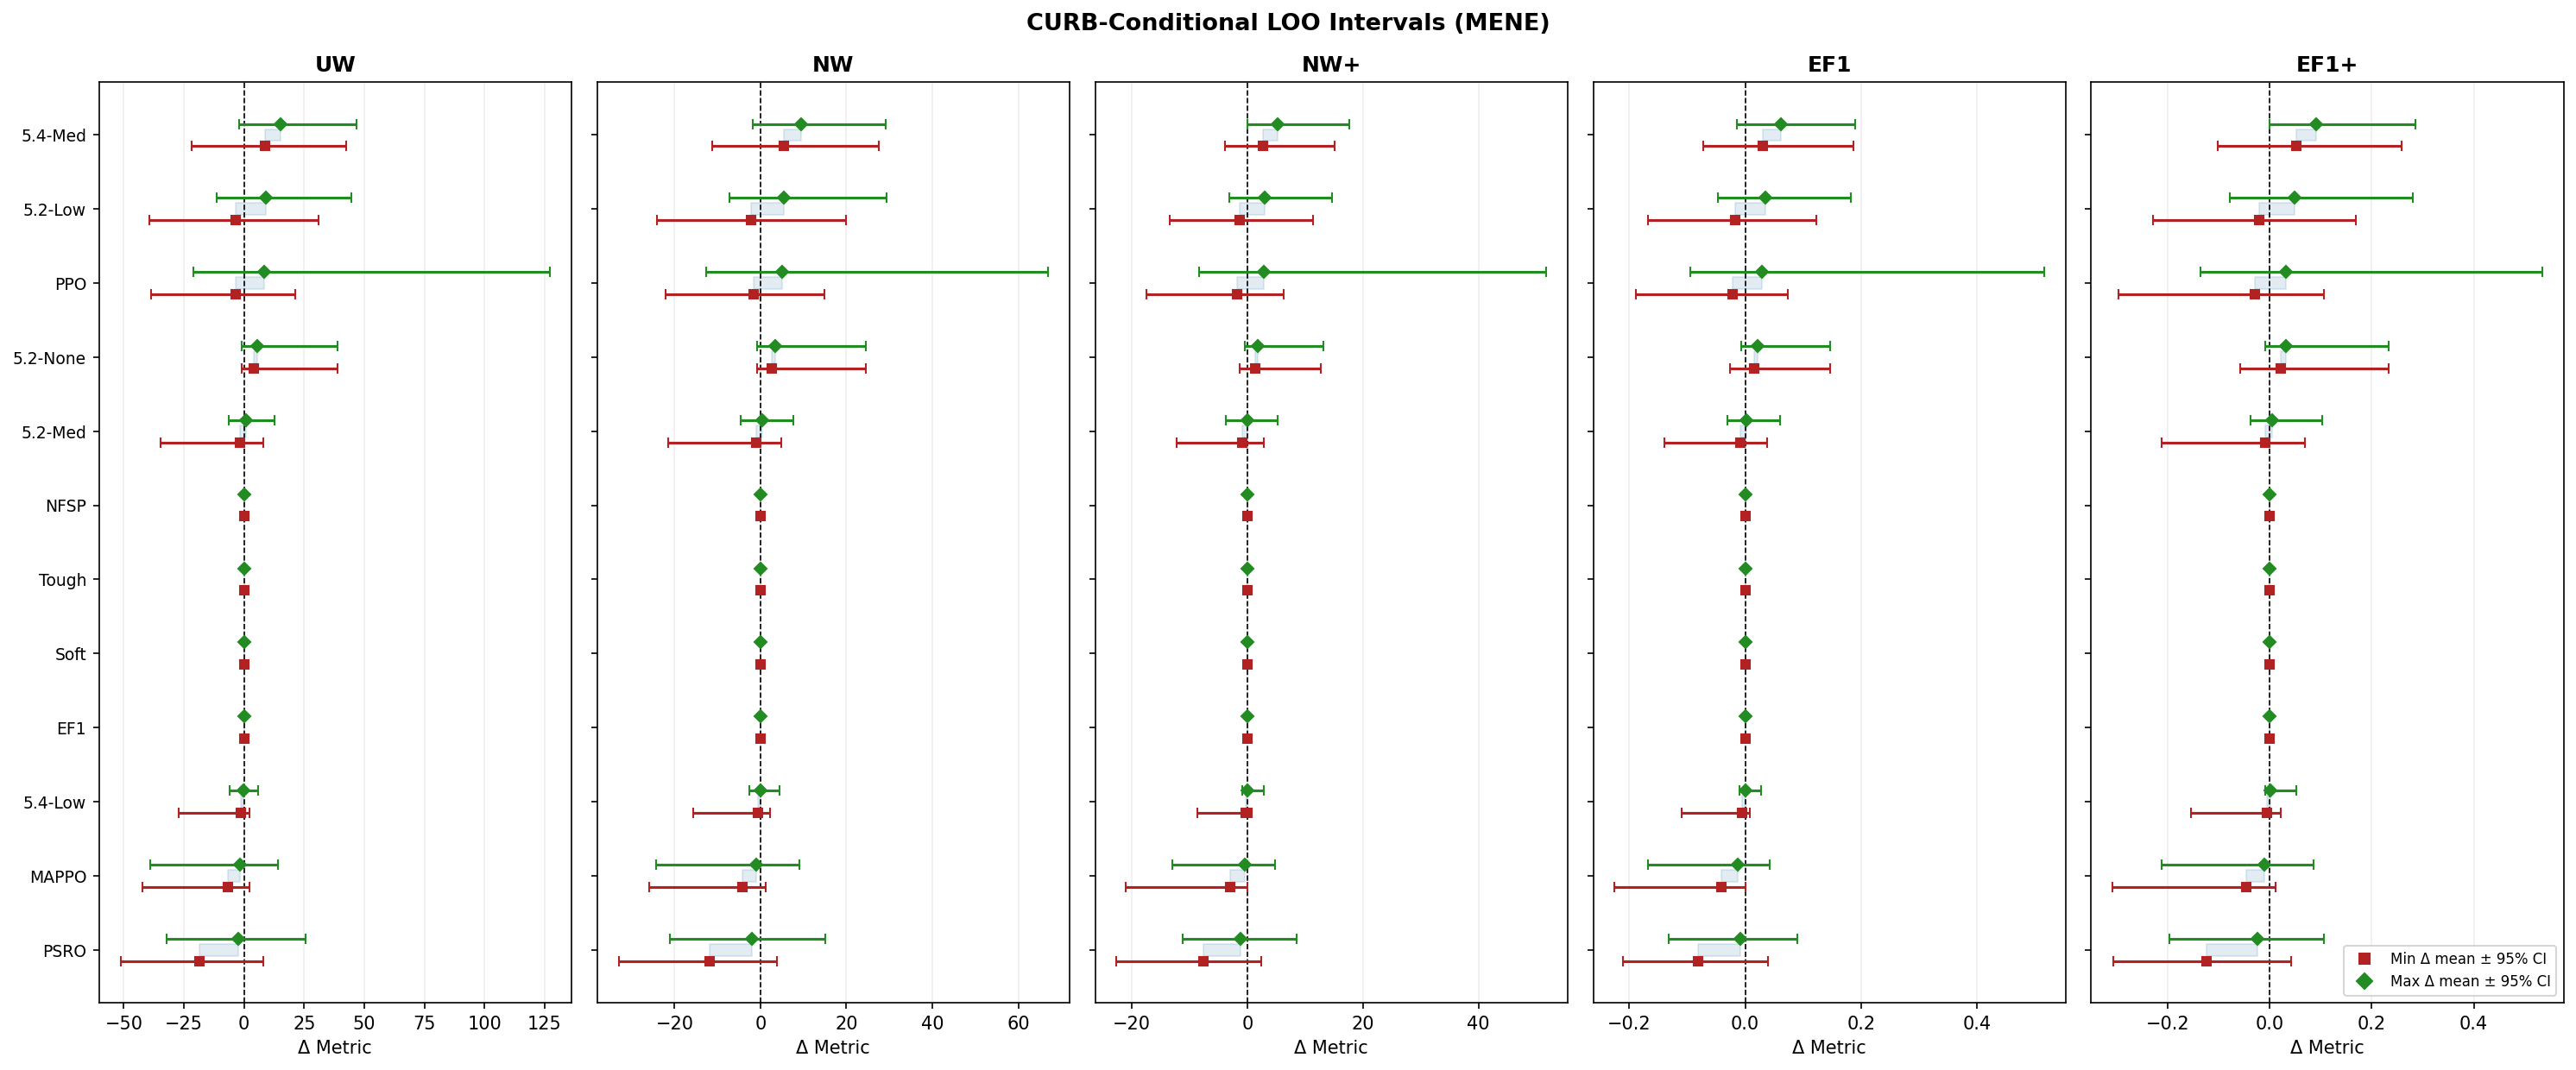
\includegraphics[width=\textwidth]{curb_loo_intervals_mene.png}
\caption{CURB-conditional LOO intervals under MENE, across bootstrap resamples of the bargaining empirical game. For each agent (rows) and metric (columns), the red square is the mean $\pm 95\%$ CI of the per-sample minimum CURB-conditional LOO effect $\underline{\Delta}$, and the green diamond is the mean $\pm 95\%$ CI of the per-sample maximum $\overline{\Delta}$. LLM strategies carry positive upper bounds; PSRO and MAPPO carry negative lower bounds.}
\label{fig:curb-mene}
\end{figure*}

\begin{figure*}[t]
\centering
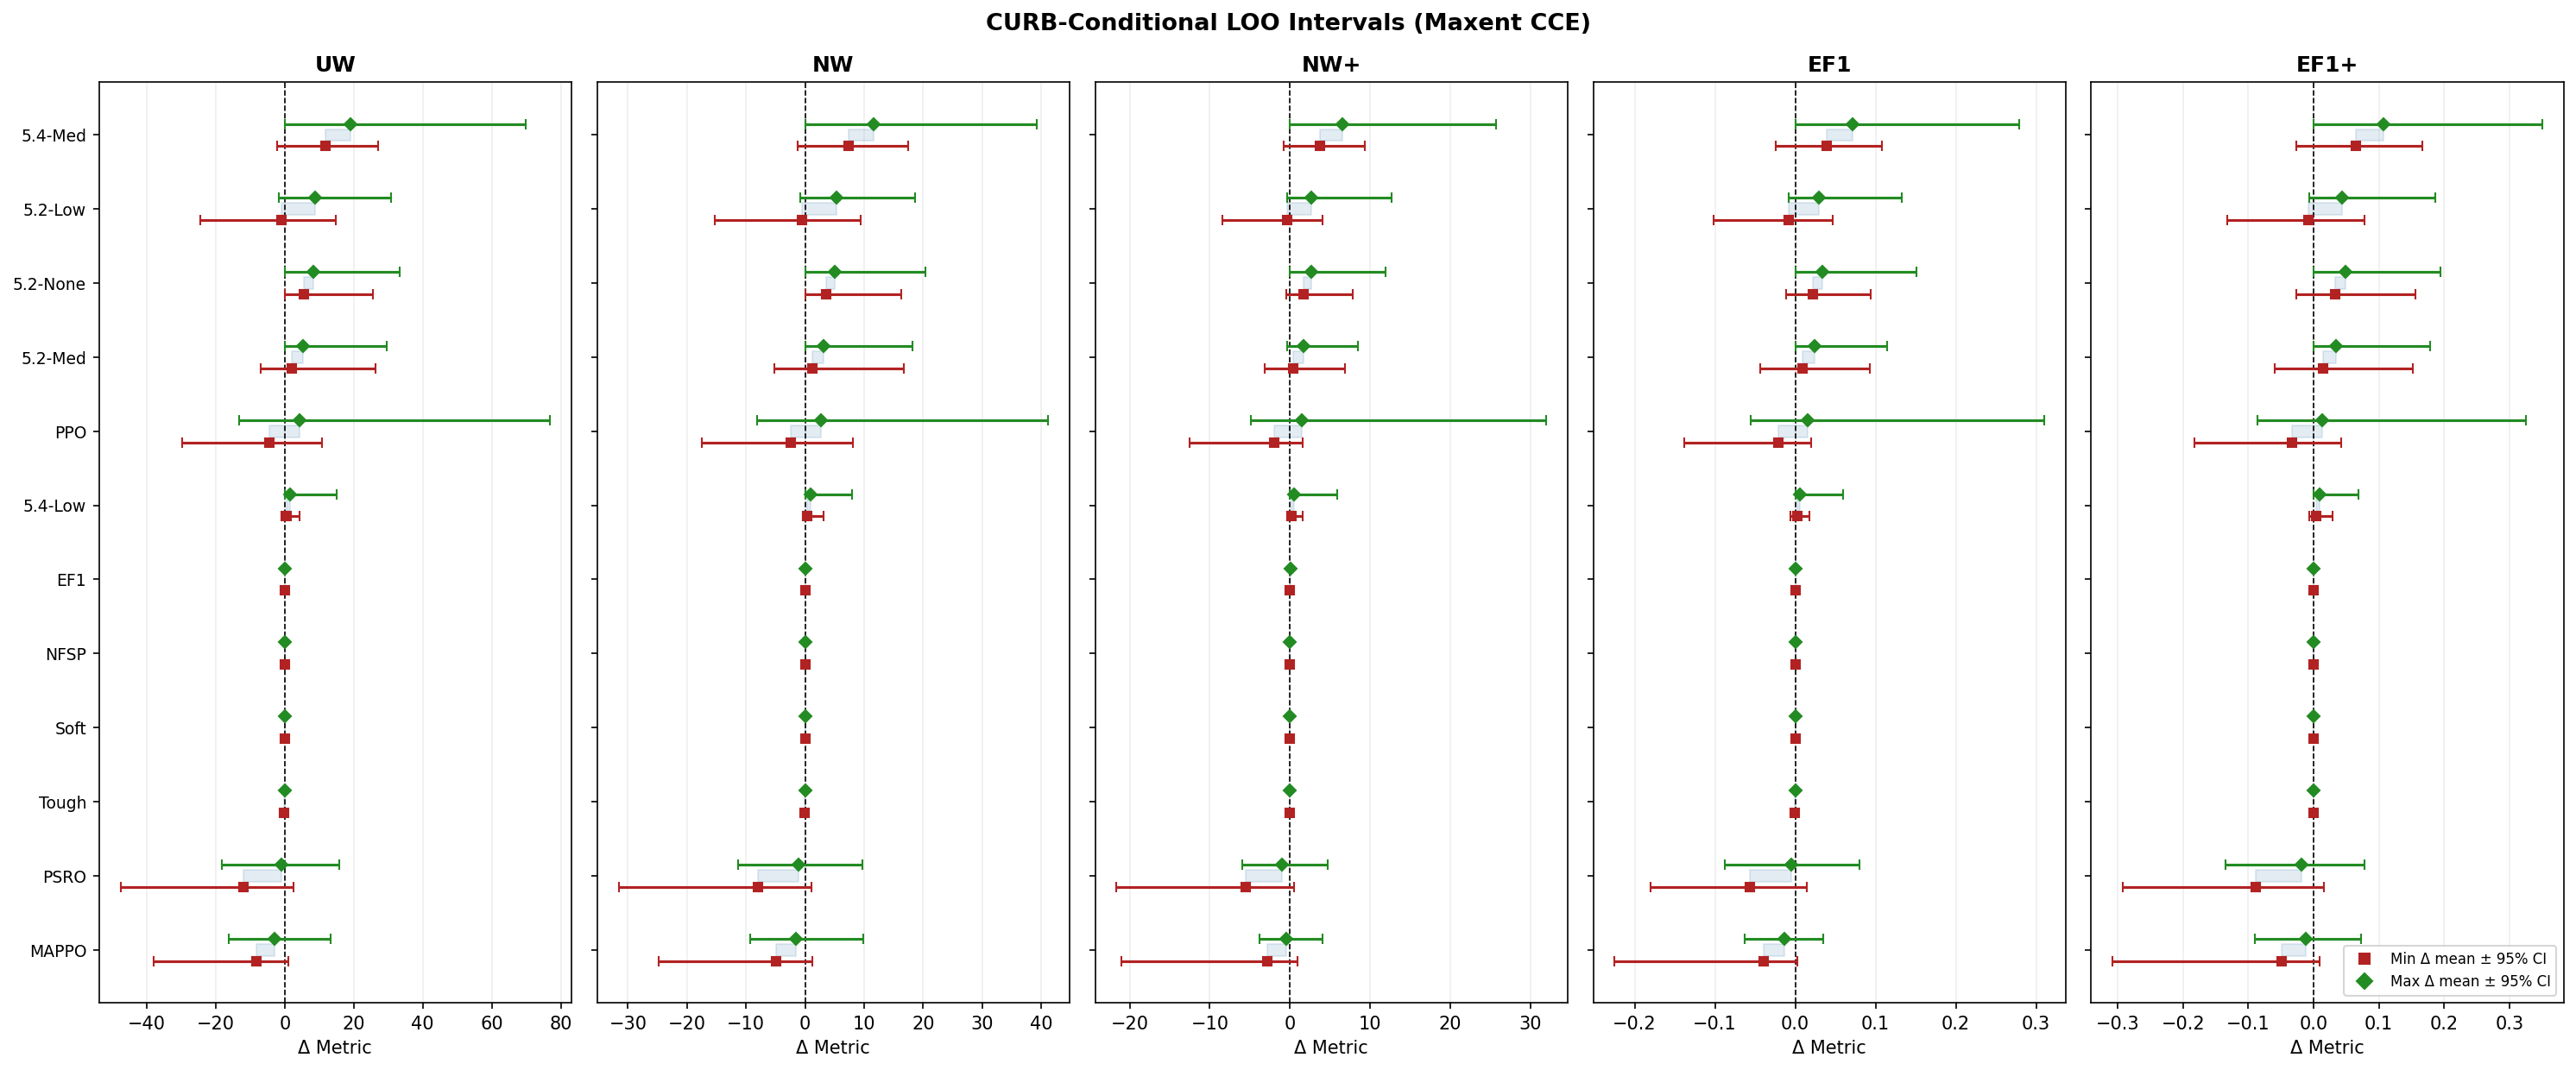
\includegraphics[width=\textwidth]{curb_loo_intervals_maxent_cce.png}
\caption{CURB-conditional LOO intervals under maximum-entropy CCE, across the same bootstrap resamples (conventions as in Figure~\ref{fig:curb-mene}). Although CCE selects a very different point equilibrium from MENE (LLM-dominated rather than RL-dominated), the interval structure---LLM strategies with positive upper bounds, PSRO and MAPPO with negative lower bounds---is preserved, evidencing the solver-robustness of the CURB-conditional analysis.}
\label{fig:curb-cce}
\end{figure*}

\section{Results}
% Closing structural ("curbset") analysis to be added here:
% CURB coverage / when CURB-conditional analysis is informative, and the PD cross-domain results.


% \subsection{Welfare Metrics}

% For a two-player symmetric empirical game with payoff matrix $M$, we evaluate the following metrics at a symmetric equilibrium $\sigma$. Each metric
% is computed as $\sigma^\top W \sigma$ where $W$ is the appropriate metric matrix.

% \textbf{Utilitarian Welfare (UW).} The sum of both players' payoffs:
% \begin{equation}
%   \text{UW}(\sigma) = \sigma^\top M \sigma + \sigma^\top M^\top \sigma
% \end{equation}

% \textbf{Nash Welfare (NW).} The geometric mean of payoffs, capturing efficiency with fairness:
% \begin{equation}
%   \text{NW}(\sigma) = \sigma^\top W_{\text{NW}} \sigma, \quad W_{\text{NW}}[i,j] = \sqrt{u_i(s_i, s_j) \cdot u_j(s_j, s_i)}
% \end{equation}

% \textbf{Nash Welfare on Advantages (NW+).} Nash welfare computed on surplus above each player's BATNA (Best Alternative to Negotiated Agreement):
% \begin{equation}
%   \text{NW+}(\sigma) = \sigma^\top W_{\text{NW+}} \sigma, \quad W_{\text{NW+}}[i,j] = \sqrt{\max(u_i - b_i, 0) \cdot \max(u_j - b_j, 0)}
% \end{equation}

% \textbf{Envy-Free up to One Item (EF1).} The frequency of outcomes satisfying the EF1 fairness criterion, where no player envies the other's
% allocation after removing at most one item:
% \begin{equation}
%   \text{EF1}(\sigma) = \sigma^\top W_{\text{EF1}} \sigma, \quad W_{\text{EF1}}[i,j] = \Pr[\text{EF1 satisfied} \mid s_i, s_j]
% \end{equation}

% \textbf{Cooperation Rate.} For iterated matrix games, the frequency of mutual cooperation:
% \begin{equation}
%   \text{Coop}(\sigma) = \sigma^\top W_{\text{Coop}} \sigma, \quad W_{\text{Coop}}[i,j] = \text{cooperation frequency between } s_i \text{ and } s_j
% \end{equation}
 

\bibliographystyle{ACM-Reference-Format} 
\bibliography{main}

%%%%%%%%%%%%%%%%%%%%%%%%%%%%%%%%%%%%%%%%%%%%%%%%%%%%%%%%%%%%%%%%%%%%%%%%

\end{document}

%%%%%%%%%%%%%%%%%%%%%%%%%%%%%%%%%%%%%%%%%%%%%%%%%%%%%%%%%%%%%%%%%%%%%%%%

